\label{mapeamento_sistematico}

Este capítulo descreve o mapeamento sistemático, método utilizado para estruturar a pesquisa da literatura. A pesquisa possibilita de identificar, avaliar e interpretar trabalhos científicos além de contribuir no estudo e na resposta da questão da pesquisa, como afirma os autores Kitchenham, Petticrew e Almeida \cite{kitchenham2007guidelines,petticrew2008systematic,de2018mapeamento}. O objetivo deste mapeamento sistemático é verificar na literatura textos correspondentes as questões definidas neste trabalho e que possam colaborar nas respostas sobre monitoramento de sistemas distribuídos.

%%%%%%%%%%%%%%%%%%%%%%%%%%%%%%%%%%%%%%%%%%%%%%%%%%%%%%%%%%%%%%%%%%%%%%%%%%%%%%%

\section{Questões de Pesquisa}
\label{questoes1e2}

Para alcançar o objetivo da pesquisa, foram levantadas algumas questões de pesquisa \textbf{(QP)}, neste trabalho serão utilizadas 2 questões, com o intuito de fornecer auxílio na fundamentação da pesquisa relacionada ao monitoramento de sistemas distribuídos, as questões são descritas as seguir. As questões têm a intensão de fornecer subsídio durante a busca de informações sobre o tema, possibilitando identificar trabalhos e experiências técnicas que já foram executadas e analisadas, como Feltrim\cite{feltrim2004abordagem} descreve em seu trabalho.

\begin{description}
\item[QP1)] Quais os estudos primários existentes na literatura que discutem os mecanismos de monitoramento 
que são aplicados a sistemas distribuídos?
\item[QP2)] Quais são as principais preocupações relativas ao monitoramento de sistemas distribuídos são mencionadas nos estudos primários?
\end{description}

%%%%%%%%%%%%%%%%%%%%%%%%%%%%%%%%%%%%%%%%%%%%%%%%%%%%%%%%%%%%%%%%%%%%%%%%%%%%%%%%

\section{Estratégia de busca}
\label{sec:stringbusca}

Para a identificação e busca dos trabalhos com maior relevância e aderência ao tema abordado e definido nas questões de pesquisa, foi criada uma \textit{string} de busca. De acordo com Keele \textit{et al.} \cite{keele2007guidelines}, a forma para a criação de uma \textit{string} de busca, é feita a partir da identificação sinônimos, abreviações e etc., e também por meio de operadores lógicos, como por exemplo, \textit{AND} e \textit{OR} que auxiliam e permitem concatenar os termos identificados, o que possibilita a elaboração de uma \textit{string}. Para a realização da pesquisa levou-se em conta os padrões e tecnologias mais comuns do mercado utilizados para o monitoramento de sistemas distribuídos juntamente com algumas palavras chave: \textit{"Monitoring Protocol"}, \textit{"Distributed Systems"}, \textit{"Monitoring"}, "\acrshort{SOA}", "\textit{web services}" e "\acrshort{ESB}". As palavras chave foram escritas em inglês para uma maior abrangência de trabalhos publicados em jornais e revistas internacionais. Diante da situação obteve-se a seguinte \textit{string} de busca: \textit{(("Protocol Monitoring" OR "Monitoring Systems") AND ("Distributed Systems"OR "SOA")) OR ( ("ESB" AND "Web Services" AND "REST"))}.

De acordo com Kitchenham \cite{kitchenham2007guidelines}, a obtenção da \textit{string} de busca, foi iniciada a pesquisa dos trabalhos e artigos científicos, as pesquisas foram realizadas nas bases de dados digitais que indexam os principais trabalhos científicos do ramo da \acrlong{TI}, para essa atividade foi utilizado um protocolo pesquisa para a execução do mapeamento sistemático, o protocolo foi separado por etapas, uma representação protocolo de pesquisa poderá ser visualizada na figura \ref{fig:etapasRSL}, a execução das etapas proporcionaram uma maior abrangência no acesso à literatura do tema pesquisado.

\begin{figure}[!ht]
\centering
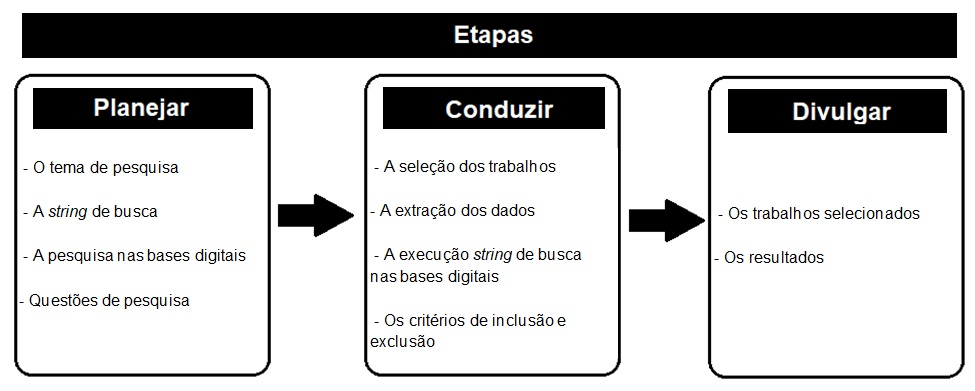
\includegraphics[width = 16cm, height=9cm]{img/etapas_RSL_final.jpg}
\caption{Etapas do \acrlong{MS}}
\label{fig:etapasRSL}
\end{figure}

Para a continuidade das atividades definidas na estratégia de busca seguindo o protocolo de pesquisa definido, a realização das consultas nas bases será feita por meio da execução da \textit{string} de busca definida. As bases selecionadas e consultadas para revisão da literatura foram:
\begin{itemize}
\item \acrlong{ACM} - \url{https://dl.acm.org/}
\item \acrlong{IEEE} - \url{https://ieeexplore.ieee.org/}
\item \acrlong{SD} - \url{https://www.sciencedirect.com/}
\item \acrlong{Scps} - \url{https://www.scopus.com/}
\item \acrlong{WoS} - \url{https://www.webofknowledge.com/}
\end{itemize}

%%%%%%%%%%%%%%%%%%%%%%%%%%%%%%%%%%%%%%%%%%%%%%%%%%%%%%%%%%%%%%%%%%%%%%%%%%%%%%%%

\section{Critérios de Inclusão e Exclusão}
\label{sec:cIncExc}
Os critérios de inclusão e exclusão foram definidos para auxiliar na seleção dos trabalhos, esse critérios auxiliam na buscar por trabalhos científicos de maior relevância e mais aderentes as questões de pesquisas definidas. Esses critérios foram utilizados em uma ferramenta de apoio que permitiu analisar os trabalhos parcialmente possibilitando incluir ou excluir da seleção os trabalhos a partir da leitura do titulo, resumo, introdução e conclusão dos trabalhos disponíveis, que foram obtidos durante a pesquisa nas bases de dados digitais.    

Os critérios de inclusão \textbf{(CI)} utilizados na seleção dos trabalhos foram:

\begin{description}

\item[CI1)] Estudo sobre monitoramento de serviços distribuídos;
\item[CI2)] Estudo sobre monitoramento de serviços em barramentos \acrshort{SOA};
\item[CI3)] Estudo sobre monitoramento de \textit{web services} pelo Protocolo \acrshort{SNMP}.
\end{description}

Os critérios de exclusão \textbf{(CE)} utilizados na seleção dos trabalhos foram:

\begin{description}
\item[CE1)]Artigos cujo foco não seja monitoramento de serviços distribuídos ou o monitoramento por Protocolo \acrshort{SNMP} monitoramento em barramentos \acrshort{SOA} ou monitoramento de \textit{web services};
\item[CE2)] Artigos publicado como \textit{Short Paper};
\item[CE3)] Mesmo Artigo publicado em locais diferentes.
\end{description}

%%%%%%%%%%%%%%%%%%%%%%%%%%%%%%%%%%%%%%%%%%%%%%%%%%%%%%%%%%%%%%%%%%%%%%%%%%%%%%%%

\section{Extração dos Dados}
A atividade de extração e seleção dos trabalhos foi dividida e realizada em quatro fases, a primeira fase foi a busca automática nas base de dados digitais com a execução da \textit{string} de busca descrita na seção \ref{sec:stringbusca}, seguindo o protocolo definido para a busca de trabalhos científicos aderentes ao tema abordado. A segunda fase foi a realização de uma pesquisa com a intenção de encontrar uma ferramenta que possibilitasse o registro e o gerenciamento dos trabalhos buscados, a terceira fase foi a seleção de forma manual para refinar a escolha dos trabalhos relacionados ao tema e a quarta foi a leitura dos trabalhos seguindo os itens definidos no protocolo para extração das informações dos trabalhos selecionados. Durante a realização da extração dos dados por meio da execução da \textit{string} de busca em cada base obteve-se vários tipos de informações sobre os dados buscados, como por exemplo, o ano da publicação do trabalho, os locais de realização dos eventos, o \acrshort{DOI} dos trabalhos publicados, além do  expressivo número de trabalhos que uma base retornou e o número significativo que outra retornou, após a consulta realizada nas bases digitais como se apresenta a seguir na tabela \ref{tabelaresultaddos}.

\begin{itemize}
\item Fase 1: Nessa fase foi realizada a busca dos trabalhos científicos nas bases digitais \acrlong{ACM}, \acrlong{IEEE}, \acrlong{SD}, \acrlong{Scps} e \acrlong{WoS}. Os trabalhos retornados foram obtidos por meio da utilização da \textit{string} de busca descrita na seção \ref{sec:stringbusca}, que após a execução da \textit{string} como meio de filtragem para a obtenção do trabalhos em cada base, obteve-se o retorno dos trabalhos relacionados com maior relevância e os mais aderentes ao tema do projeto. A busca nas bases de dados foi possível por causa da definição das palavras e textos registrados na \textit{string} de busca, ocasionando o refinamento da busca dos trabalhos totalizando o número de 3.227 trabalhos publicados, que foram retornados após a pesquisa, conforme o registro na tabela \ref{tabelaresultaddos}.

\begin{table}[!ht]
\centering
\caption{Trabalhos retornados por base de dados digital}
\label{tabelaresultaddos}
    \begin{tabular}{|c|c|}
        \hline
        \multicolumn{2}{|c|}{\textbf{Fase 1}} \\ \hline
        \textbf{\begin{tabular}[c]{@{}c@{}}Base de dados\end{tabular}} & \textbf{\begin{tabular}[c]{@{}c@{}}Total\end{tabular}} \\ \hline
        \acrlong{ACM}  & 86 \\ \hline
        \acrlong{IEEE}  & 68 \\ \hline
         \acrlong{SD} & 2492 \\ \hline
         \acrlong{Scps} & 515 \\ \hline
         \acrlong{WoS} & 66 \\ \hline
    \end{tabular}
\end{table}

\item Fase 2: Após a conclusão da fase 1, que foi a realização da busca dos trabalhos nas bases científicas foi detectada a necessidade de utilização de uma ferramenta que possibilitasse um melhor controle e gerenciamento dos trabalhos científicos que foram retornados das bases. A necessidade surgiu por causa do grande volume de trabalhos retornados, que durante a realização do processo de extração poderia ocasionar a perda do conhecimento ou confusão no entendimento do problema, devido a não organização dos dados obtidos pela leitura dos trabalhos. A ideia foi identificar uma ferramenta capaz de auxiliar no registro de informações obtidas na extração trabalhos buscados. Nesse seguimetos os autores Almeida e Zamboni \textit{et al.} \cite{de2002pesquisas,zamboni2010start} descrevem, depois de uma pesquisa na literatura, conversar com professores e grupos de alunos sobre ferramentas com a finalidade que compõem o processo metodológico para auxílio na extração de dados, a ferramenta selecionada para a execução do trabalho foi o \acrshort{StArt}\textsuperscript{\textregistered}.  

\item Fase 3: Após a filtragem e extração dos trabalhos das bases de dados cientificas, e a seleção da ferramenta de apoio para o auxílio no processo de extração dos dados, foi feita a exportação dos metadados dos trabalhos retornados de cada base digital em formato BibTex\textsuperscript{\textregistered}, como afirma o autor Chomsky \cite{chomsky1969linguistica}, após a exportação desses dados foi realizada a importação desses dados na ferramenta \acrshort{StArt}\textsuperscript{\textregistered}. Na ferramenta foi realizada a importação e em seguida a organização por base cientifica. Duratne a leitura dos títulos e resumos ou a leitura das introduções e conclusões dos trabalhos importados foram executados os critérios para a seleção dos trabalhos, com os tópicos de inclusão e exclusão descritos na seção \ref{sec:cIncExc}, para a realização da seleção dos trabalhos para a leitura final. De acordo com Petersen \textit{et al.} \cite{petersen2008systematic} a execução desse método, visa minimizar a leitura completa de trabalhos que necessariamente não tratam do assunto. Após a utilização dos critérios de inclusão e exclusão dos trabalhos foi possível selecionar os trabalhos mas aderentes ao tema do trabalho para a leitura. A figura \ref{fig:fase3Criterios} representa a execução dos critérios permitindo identificar os trabalhos que por meio da leitura completa, possam ajudar nas respostas das questões de pesquisa.  


\begin{figure}[!ht]
\centering
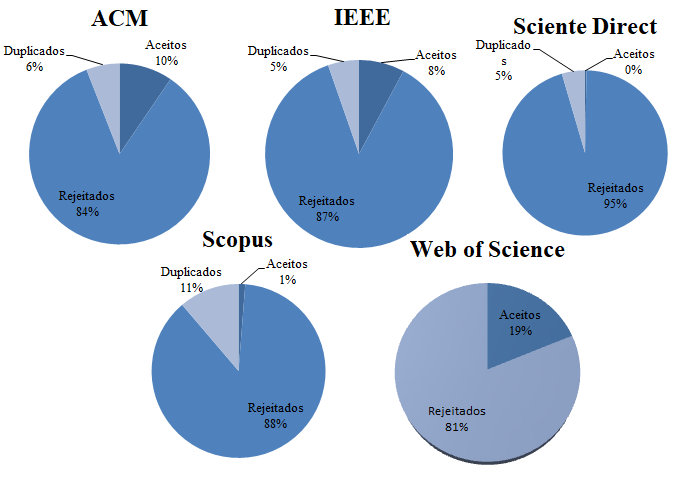
\includegraphics[width = 13cm, height=10cm]{img/Classificacao_FASE_3_CI_e_CE.png}
\caption{Resultado da Fase 3 classificação (CI e CE) em porcentagem.}
\label{fig:fase3Criterios}
\end{figure}

\item Fase 4: Após a realização da classificação dos trabalhos científicos retornados por meio do processo metodológico que permitiu a utilização dos critérios de inclusão e exclusão obteve-se o total de 51 trabalhos selecionados para que fosse realizada a extração dos dados desses trabalhos, em seguida foi iniciada a 4º fase que possibilitou a observação mais aprofundada nos trabalhos e a leitura completa. Com a leitura completa dos trabalhos, a ferramenta \acrshort{StArt}\textsuperscript{\textregistered} foi utilizada para a continuidade do mapeamento sistemático, onde nessa fase foram incluídos nos formulários da ferramenta atributos definidos no protocolo de pesquisa e especificamente registrados como "campos para a extração dos dados", que permitiu a avaliação dos trabalhos por meio de uma a análise empírica, onde as devidas anotações e classificações de cada trabalho foi registrada na ferramenta, o que permitiu catalogar o trabalho para facilitar a recuperação dos pontos mais importantes de uma forma mais rápida e precisa assim como identificar os trabalhos mais relevantes e aderentes as questões de pesquisa. Após a leitura, a realização de registros e análise dos trabalhos obteve-se um refinamento na classificação, onde foi alcançada a marca de 22 trabalhos extraídos e selecionados dos 51 trabalhos que foram selecionado nessa fase. Os 22 trabalhos selecionados estão na tabela \ref{tabelaresultadosAnalise}, os trabalhos selecionados após a extração contribuíram para a fundamentação teórica do tema, possibilitando aprimorar o conhecimento para responder as questões de pesquisa. 

\end{itemize}


\begin{longtable}{|l|l|l|}
\caption{Trabalhos selecionados}
\label{tabelaresultadosAnalise}
\hline
\endhead
\begin{tabular}[c]{@{}l@{}}[Ts-1]  Abousharkh, Maha and \\ Mouftah, Hussein. \\   Service Oriented \\ Architecture-based\\   Framework for WBAN-\\ enabled Patient \\   Monitoring System \cite{abousharkh2011service}.\end{tabular} & \begin{tabular}[c]{@{}l@{}}[Ts-9] Abdu, Hasina and \\ Lutfiyya,\\   Hanan and Bauer, \\ Michael A. \\ Monitoring Overhead \\ in Distributed\\  Systems:  Visualization\\  and Estimation \\ Techniques \cite{abdu1996monitoring}.\end{tabular} & \begin{tabular}[c]{@{}l@{}}[Ts-17] Casola, Valentina \\ and   Gaglione, Andrea \\ and Mazzeo, Antonino. \\ SeNsIM-Web: a Service \\ Based  Architecture for \\ Sensor Networks \\ Integration \cite{casola2009sensim}.\end{tabular} \\ 
\hline
\begin{tabular}[c]{@{}l@{}}[Ts-2]  Abdu, Hasina and \\ Lutfiyya, Hanan L. \\ and Bauer, Michael A. \\ An Investigation of\\ Monitoring Configurations \cite{abdu1995investigation}.\end{tabular} & \begin{tabular}[c]{@{}l@{}}[Ts-10] Wang, Bo and \\ Song, Ying and\\   Sun, Yuzhong and\\  Liu, Jun. \\ Improvements\\  to online distributed \\ monitoring systems \cite{wang2016improvements}.\end{tabular} & \begin{tabular}[c]{@{}l@{}}[Ts-18] Kotsopoulos, \\ Konstantinos  and Lei, \\ Pouwan and Hu, Yim \\ Fun. A SOA-based \\ information \\ management model \\ for  Next-Generation \\ Network \cite{kotsopoulos2008soa}.\end{tabular} \\ 
\hline
\begin{tabular}[c]{@{}l@{}}[Ts-3]  Cirstoiu, Catalin C. \\ and Grigoras, \\ Costin C. and Betev, \\ Latchezar L. and\\   Costan, Alexandru A.\\  and Legrand, \\ Iosif Charles. \\ Monitoring, Accounting \\ and  Automated \\ Decision Support for the \\ Alice Experiment \\ Based on the MonALISA \\ Framework \cite{cirstoiu2007monitoring}.\end{tabular} & \begin{tabular}[c]{@{}l@{}}[Ts-11] Nagorny, Kevin\\  and  Harrison, \\ Robert and Colombo,\\  Armando Walter \\ andKreutz, Gerhard. \\ A Formal Engineering \\ Approach for Control \\ and Monitoring \\ Systems in a \\ Service-Oriented \\ Environment \cite{nagorny2013formal}.\end{tabular} & \begin{tabular}[c]{@{}l@{}}[Ts-19] Smith, Garry \\ and Baker,\\   Mark. A Flexible\\  Monitoring and \\ Notification System \\ for Distributed  \\ Resources \cite{smith2008flexible}.\end{tabular} \\ 
\hline
\begin{tabular}[c]{@{}l@{}}[Ts-4]  Repantis, Thomas and\\  Cohen, Jeff and \\ Smith, Scott and Wein, \\ Joel. Scaling a\\   Monitoring Infrastructure \\ for the Akamai Network \cite{repantis2010scaling}.\end{tabular} & \begin{tabular}[c]{@{}l@{}}[Ts-12] Ghorbani, Shirin \\ and Du, Weichang. \\ Personal Health \\ Service Framework \cite{ghorbani2013personal}.\end{tabular} & \begin{tabular}[c]{@{}l@{}}[Ts-20] Lee, JS and \\ Hsu, PL. Design\\ and implementation \\ of the SNMP agents \\ for remote monitoring \\ andcontrol via  UML\\  and Petri nets \cite{lee2004design}.\end{tabular} \\ 
\hline
\begin{tabular}[c]{@{}l@{}}[Ts-5]  Sedayao, Jeff. \\ Implementing and \\ Operating an Internet \\ Scale Distributed\\   Application Using \\ Service Oriented \\ Architecture Principles \\ and Cloud\\   Computing \\ Infrastructure \cite{sedayao2008implementing}.\end{tabular} & \begin{tabular}[c]{@{}l@{}}[Ts-13] Penteado, Mauricio \\ G. and Trevelin, Luis \\ Carlos. JMonitor: A \\ monitoring tool for\\  distributed systems \cite{penteado2012jmonitor}.\end{tabular} & \begin{tabular}[c]{@{}l@{}}[Ts-21] Feng, JQ and \\ Buse, DP and\\  Wu, QH and Fitch, J. \\ Distributed mobile \\ communication \\ base station diagnosis \\ and monitoringusing \\ multi-agents \cite{feng2002distributed}.\end{tabular} \\ 
\hline
\begin{tabular}[c]{@{}l@{}}[Ts-6]  Subramanyan, Rajesh \\ and Miguel-Alonso, José \\ and Fortes, José A. \\ B. A Scalable  SNMP-\\ based Distibuted \\ Monitoring System \\ for Heterogeneous \\ Network Computing \cite{subramanyan2000scalable}.\end{tabular} & \begin{tabular}[c]{@{}l@{}}[Ts-14] Patrut, Bogdan \\ and Tomozei,\\  Cosmin. Agent \\ Technology in \\ Monitoring Systems \cite{puatruct2010agent}.\end{tabular} & \begin{tabular}[c]{@{}l@{}}[Ts-22] P. Qi-rui and W. \\ Cheng and\\   W. Jing and L. Jun \\ and L. Qing and S. \\ Bei-en. An \\ authentication and \\ authorization solution \\ supporting SOA-based \\ distributed systems \cite{qi2010authentication}.\end{tabular} \\ 
\hline
\begin{tabular}[c]{@{}l@{}}[Ts-7]  Joyce, Jeffrey and \\ Lomow, Greg \\ and Slind, Konrad and \\ Unger, Brian. \\ Monitoring  Distributed \\ Systems \cite{joyce1987monitoring}.\end{tabular} & \begin{tabular}[c]{@{}l@{}}[Ts-15] Phan, Raphael \\ C. -W.  Cryptanalysis \\ of the application \\ secure alternative \\ to SNMP (APSSNMP) \cite{phan2009cryptanalysis}.\end{tabular} &  \\ 
\hline
\begin{tabular}[c]{@{}l@{}}[Ts-8] P.  Yan and J. Guo. \\ Researching and \\ Designing the \\ Architecture of \\ E-government\\   Based on SOA \cite{yan2010researching}.\end{tabular} & \begin{tabular}[c]{@{}l@{}}[Ts-16] Hirate, Yu and \\ Yamana,\\   Hayato. Profiling Node \\ Conditions of Distributed \\ System \\ with Sequential\\   PatternMining \cite{hirate2009profiling}.\end{tabular} &  \\ \hline
\end{longtable}

%%%%%%%%%%%%%%%%%%%%%%%%%%%%%%%%%%%%%%%%%%%%%%%%%%%%%%%%%%%%%%%%%%%%%%%%%%%%%%%%

\section{Resultados}
Após a realização da pesquisa dos trabalhos nas bases digitais, a seleção e extração dos trabalhos para a leitura, nesta seção por meio da utilização do mapeamento sistemático será possível responder as questões de pesquisa descritas na seção \ref{questoes1e2} de forma fundamentada pelos trabalhos científicos obtidos por meio de resumos referentes as questões. A leitura dos trabalhos ampliou o conhecimento sobre o tema e permitiu a identificação e apresentação dos seguintes itens, para utilizá-los como base para a execução do projeto, são eles:
\begin{itemize}
\item Monitoramento de sistemas distribuídos
\item \textit{Web services}
\item Agentes de monitoramento
\item Protocolo \acrshort{SNMP}
\item Armazenamento das Informações monitoradas
\item Desempenho
\end{itemize}

\subsubsection{QP1) Quais os estudos primários existentes na literatura que discutem os mecanismos de monitoramento que são aplicados a sistemas distribuídos?}

\subsubsection{Monitoramento de Sistemas Distribuídos}
Na realização da pesquisa nos trabalhos selecionados foi identificada a necessidade do monitoramento de sistemas distribuídos, devido a grande quantidade de  aplicações, dispositivos e web services em funcionamento, e que normalmente não possuem acompanhamento durante o funcionamento. Em \cite{cirstoiu2007monitoring} descrito sobre o monitoramento de sistemas distribuídos e da utilização das API's para a comunicação de aplicativos e a preocupação com o baixo acoplamento dessas ferramentas. Em outro trabalho \cite{joyce1987monitoring} é descrito sobre a importância do monitoramento de sistemas distribuídos, e a utilização testes de programas de para a verificação dos sistemas monitorado. No entanto em \cite{abdu1996monitoring} é descrito o quanto é complexo o gerenciamento do monitoramento de sistemas distribuídos, sendo necessário a utilização de técnicas e métricas para obtenção dos resultados coletados, por conta da grande quantidade de informações geradas pelo monitoramento.  

\subsubsection{Web Services}

Os trabalhos \cite{patil2012remote,casola2009sensim} apresentam como a flexibilidade e agilidade no desenvolvimento de \textit{web services}, podem trazer resultados imediatos para as aplicações, suas características que facilitam a integração dos serviços e sistemas e como é fácil a integração de ambientes com os padrões da Indústria e protocolos como SOAP, HTTP e etc., porém a facilidade abre uma preocupação referente a segurança das aplicações, principalmente no que tange a integridade e confidencialidade dos dados, uma dessas ameaças é o \textit{SQL Injection}. 

\subsubsection{Agentes de Monitoramento}

Agentes de monitoramento podem ser um dispositivo ou um software, esses podem ser utilizados para realizar a comunicação ou notificação do monitoramento de outros dispositivos ou sistemas distribuídos. Em \cite{smith2008flexible} é descrito sobre a utilização e comparação de ferramentas(\textit{plugins}) que funcionam como agentes de monitoramento de sistemas distribuídos e também da arquitetura definida para o gerenciamento e acompanhamento. No trabalho \cite{puatruct2010agent} é descrito sobre o experimento com informações metacognitivas que proporcionaram 12 definições para a identificação de agentes inteligentes, propostas para a definição de um agente ou Super agente, e como eles podem monitorar sistemas para realização de comunicação homem-máquina.

\subsubsection{Protocolo SNMP}
\label{snmpDescription}

Em \cite{deGeus} é descrita a definição de um modelo computacional configurável para o gerenciamento e monitoramento de redes, servidores, armazenamento, aplicações e serviços com a utilização do protocolo SNMP para realização de coleta de informações para que sejam criadas métricas onde se possa obter resultados satisfatórios dos serviços disponibilizados. No  trabalho \cite{daSilva} são explicadas informações do protocolo SNMP, como o seu funcionamento, sua utilização , Agente(processo), os tipos de Agente, o Gerente que é uma aplicação, em execução em uma estação de gerenciamento, as operações do protocolo, como por exemplo, \textit{GetRequest, 	GetNextRequest,  GetResponse,  SetRequest  e Trap} e também sobre as ferramentas de monitoramento que são compatíveis com o protocolo, inclusive em \cite{Fraga} é destacado que o protocolo SNMP tem sido o principal protocolo utilizado para gestão e monitoramento de redes. Entretanto, em \cite{deMello} são descritos e identificados alguns pontos fracos do protocolo \acrshort{SNMP}. Apesar  de  seu  nome,  \textit{"Simple  Network  Management  Protocol"},  o  SNMP  é  um protocolo  relativamente  complexo  para  implementar.  Também,  o  SNMP  não  é  um protocolo muito eficiente. Nos trabalhos \cite{phan2009cryptanalysis,subramanyan2000scalable} também são relatados alguns pontos fracos como a vulnerabilidade presente no SNMPv1 , desempenho e falta de escalabilidade.

\subsubsection{QP2) Quais são as principais preocupações relativas ao monitoramento de sistemas distribuídos são mencionadas nos estudos primários?}

\subsubsection{Armazenamento das Informações Monitoradas}

O Monitoramento dos sistemas distribuídos quando implementados geram informações durante a execução, essas informações são importantes para acompanhar o funcionamento de sistemas distribuído e \textit{web services}. No trabalho \cite{phan2009cryptanalysis} é descrito sobre a importância da coleta dessas informações e a coleta em larga escala utilizando instruções e comandos SQL. Porém devido ao grande número de sistemas distribuídos monitorados e a grande quantidade de informações geradas por meio do monitoramento, nos trabalhos \cite{abdu1996monitoring,hirate2009profiling} são apresentadas as técnicas para mensurar a sobrecarga gerada pela quantidade de informações e padrões de mineração dos dados armazenados.  

\subsubsection{Desempenho}

O trabalho \cite{wang2016improvements} apresenta algoritmos de compactação de dados, para a realização de transferência dos dados de modo otimizado, devido a grande quantidade de informações geradas durante o monitoramento dos sistemas distribuídos. Nesse trabalho foram realizados vários testes, incluído conversão de formatos, como por exemplo, arquivos XML. Em \cite{kotsopoulos2008soa} é descrito o motivo da não utilização do protocolo SNMP, por conta de algumas limitações, como por exemplo, a escalabilidade e eficiência. 

\section{Síntese do Capítulo}

Este capítulo apresenta a execução do mapeamento sistemático utilizado para a realizar a pesquisa da literatura e identificar nos trabalhos científicos, dados e informações relacionadas ao monitoramento de sistemas, ao protocolo de monitoramento \acrshort{SNMP} e ferramentas de monitoramento, possibilitando a fundamentação para a implementação do projeto de monitoramento dos serviços do barramento Erlangms com a utilização do protocolo \acrshort{SNMP} para a integração com ferramentas de monitoramento. O protocolo \acrshort{SNMP} foi identificado como o a solução para a implementação do projeto ,visto que a atualmente o \acrshort{CPD} já utiliza, pois  possui ferramentas de monitoramento que realizam o monitoramento de \textit{softwares} e ativos de rede, por meio do protocolo. 

%%%%%%%%%%%%%%%%%%%%%%%%%%%%%%%%%%%%%%%%%%%%%%%%%%%%%%%%%%%%%%%%%%%%%%%%%%%%%%%%%%%%%